\chapter{SonoScape Analyse}
Wie schon in Komponentendiagram \ref{fig:Komponentendiagramm} zu sehen ist, soll das SonoScape den Bildschirminhalt zuerst in Echtzeit abfilmen. Danach soll jedes einzelne Bild komprimiert werden, weil die zu übertragenen Daten möglichst klein sein sollten damit so viele Bilder pro Sekunde wie möglich an den Client geschickt werden können.\\
Um die oben genannten Punkte mit dem SonoScape realisieren zu können, muss das Gerät, insbesondere das Betriebssystem und darauf aufbauende Strukturen, analysiert werden. Denn sobald das Gerät gestartet wird, öffnet es ohne weitere  Benutzerinteraktionen zuzulassen, eine Software für die Ultraschallbehandlung. Im Kontext der Analyse des Gerätes und der Manipulation muss eine Möglichkeit gefunden werden, vollständigen root Zugriff \footnote{root Zugriff bedeutet alle Rechte über alle Dateien und Skripte auf dem System zu besitzen.} auf das System zu erlangen.\\ 
Ein möglicher Ansatz zum Ausführen von zusätzlicher Software und Treibern umfasst den Zugriff auf das BIOS-System des Ultraschallgerätes. Durch den Zugriff auf das BIOS-System kann ein angepasstes Betriebssystem gestartet und der Festplatteninhalt analysiert werden. Dazu ist allerdings ein Passwort gefragt, welches Prof. Kukuk nach Rücksprache der herstellenden Firma erhalten hat. Mit diesem Passwort war es möglich per USB-Stick ein alternatives Betriebssystem zu laden. Konkret wurde Ubuntu 10.04 32 bit gebootet ,da das SonoScape ebenfalls ein Ubuntu 10.04 in etwas veränderter Form als Bootsystem benutzt. Verändert heißt in diesem Fall, dass ein custom Linux System entworfen wurde. Dieses System verbraucht relativ wenig Speicher und hat dementsprechend nur wenige Funktionen. Deswegen fehlen auch wichtige Kommandozeilen Befehle und vieles mehr, weil diese nicht für die elementaren Funktionen des Ultraschallgerätes benötigt werden.\\
Da es durch das BIOS Passwort möglich ist das System genauer zu untersuchen und zu manipulieren, muss sichergestellt werden, dass das System nach der Analyse weiterhin ordnungsgemäß funktioniert. 
\clearpage
\begin{large}
\textbf{Sicherung}\\\\
\end{large}
Um das SonoScape zu analysieren müssen verschiedene Ansätze ausgetestet werden. Da bei dem Testen der Ansätze Veränderungen am System vorgenommen werden, wurde zuerst eine Sicherung des ursprünglichen Betriebssystems angelegt. So ist gewährleistet, dass im schlimmsten Fall eine Sicherungskopie existiert, um die Änderungen rückgängig machen zu können. Die Sicherung wurde mit dem dd\footnote{Der dd Befehl ist standardmäßig im Linux Kernel enthalten und kann den Festplatteninhalt blockweise kopieren. } Befehl unter Linux durchgeführt. Mit diesem wird eine gesamte Festplatte Block für Block auf ein anderes Speichermedium übertragen.\\\\
%\section{Betriebssystemanalyse}
Im Rahmen der Betriebssystemanalyse sind einige Probleme aufgetreten. Zum einen war das häufige hoch und runter fahren des SonoScape Gerätes sehr zeitaufwändig. Des weiteren war es nicht möglich ein deutsches Tastatur Layout einzustellen, was bei diversen Kommandozeilen Befehlen zu starken Verzögerungen in der Eingabe geführt hat. Dazu kam der hohe Wert des Gerätes, weswegen äußerste Vorsicht bei der Benutzung geboten war.\\
Aus diesen Gründen wurde das image\footnote{Blockweise Kopie des Festplatteninhalts}, also das Ergebnis der Sicherung, auf eine virtuelle Maschine übertragen. So wurden alle genannten Probleme gelöst und zusätzlich die Möglichkeit, geschaffen mit mehreren Computern parallel an der Analyse zu arbeiten. Dazu kam die Möglichkeit eine weitere virtuelle Maschine einzurichten, entsprechend des Betriebssystems des SonoScape wurde Ubuntu 10.04 32 bit für die zweite virtuelle Maschine gewählt.\\
\begin{wrapfigure}[11]{l}{0.33\textwidth}
\vspace{-19pt}
\centering
\includegraphics*[width =0.33\textwidth]{Sonoscape_Analyse/Anzahl_Festplatten}
\caption{{\small Übersicht über die 4 Partitionen der Festplatte des SonoScape Gerätes}}
\label{fig:Festplatte}
\end{wrapfigure}
Über die Software VirtualBox kann der Festplatteninhalt eines images, wie vom SonoScape image, innerhalb der virtuellen Maschine verfügbar gemacht werden. Das bedeutet, dass es dadurch möglich ist mit dem Ubuntu Betriebssystem, auf den Festplatteninhalt der virtuellen Box ,indem das SonoScape simuliert wird, zuzugreifen. Genauer gesagt kann herausgefunden werden warum ein Benutzer keine Interaktionsmöglichkeiten, abgesehen von der Bedienung der Ultraschallsoftware, mit dem System hat.\\
In der virtuellen Ubuntu Maschine kann nun die Partitionierung, Größe und der Inhalt der einzelnen Partitionen gesehen und auch manipuliert werden, siehe Abbildung \ref{fig:Festplatte}. Da das dieselben Daten sind die auch von der virtuellen SonoScape Maschine benutzt werden, kann das Verhalten nicht nur analysiert, sondern auch direkt verändert werden.
Zum Beispiel kann das direkte starten der Ultraschallsoftware unterbunden werden, vorher andere Programme gestartet werden wie ein Programm um den Bildschirm mitzuschneiden oder aber einfach eine Konsole geöffnet werden.
%\checkheight{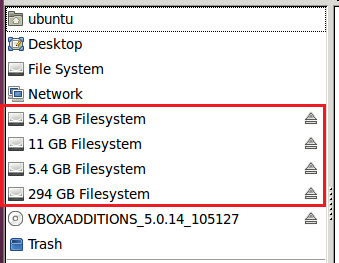
\includegraphics[width=0.9\linewidth]{Sonoscape_Analyse/Anzahl_Festplatten}}
\section{System Struktur}
Damit das System ordnungsgemäß manipuliert werden kann, ohne die Kernfunktionalität zu beschädigen, muss erst entschlüsselt werden wie genau das System aufgebaut ist. Dazu ist es wichtig den eigentlichen boot Vorgang zu verstehen, denn dieser ist elementarer Bestandteil des angepassten Betriebssystems.\\\\
\begin{large}
\textbf{Initramfs}\\\\
\end{large}
Das SonoScape Gerät benutzt das initramfs (initial ram filesystem) Konzept. Im Grund genommen wird während des bootens eine bestimmte Datei in den Arbeitsspeicher geladen und als root Dateisystem gemountet. Dieses Vorgehen hat viele Vorteile gegenüber dem klassischem boot Vorgang. Erstens wird die Größe des Kernels erheblich reduziert. Dadurch wird es leichter einen schlanken, übersichtlichen Kernel zu benutzen, der ausschließlich Kernfunktionalität übernimmt. 
\begin{wrapfigure}{r}{0.26\textwidth}
\centering
\includegraphics*[width =0.26\textwidth]{Sonoscape_Analyse/initramfs}
\caption{{\small Inhalt des RAM Dateisystems}}
\label{fig:RAM_Dateisystem}
\end{wrapfigure} 
\begin{figure}[h]
	\centering
	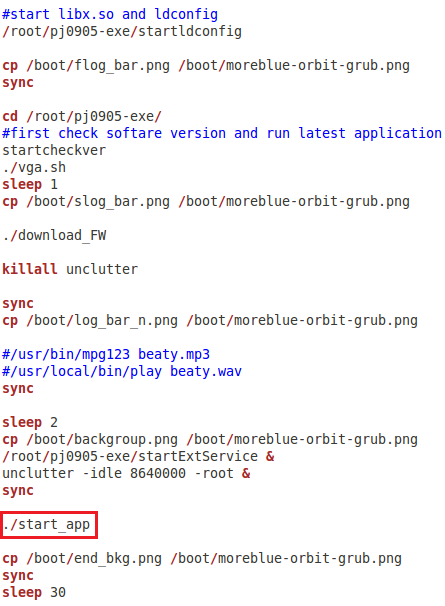
\includegraphics[width=0.5\textwidth]{Sonoscape_Analyse/run_all_app}
	\caption{Auszug aus dem run all app Skript}
	%\vspace{-1.5em}
	\label{fig:run_all_app}
\end{figure}
Zweitens ist es leichter den boot Prozess zu modifizieren, wie es auf dem SonoScape Gerät getan wurde. Zusätzliche boot Logik kann nun einfach über das initramfs hinzugefügt werden, ohne den eigentlich Kernel zu modifizieren\footcite{initframe}.
Die Logik des initramfs heißt Casper und befindet sich in einer 5,4GB großen Parition (siehe Abbildung \ref{fig:RAM_Dateisystem}), die nicht als logisches Laufwerk gemountet wird, sondern während des boot Prozesses als Arbeitsspeicherdateisystem. Sollten innerhalb dieses RAM\footnote{random access memory, Arbeitsspeicher auf deutsch} Dateisystems Änderungen vorgenommen werden, sind diese nach dem nächsten Neustart nicht persistent gespeichert, sodass Installationen von jeglicher Software revidiert werden. Trotzdem ist es möglich Software zu installieren und für die aktuelle Sitzung zu benutzen, die Software muss dementsprechend auch mit jedem Neustart des Systems neu installiert werden.

Das RAM Dateisystem modifiziert den boot Vorgang nun so, dass bestimmte, vom Hersteller generierte  Skripte, ausgeführt werden. Dazu wird die 11GB Partition als persistente Festplatte gemountet, denn auf dieser befinden sich die zusätzlichen Skripte.\\
Diese Skripte steuern, ergänzen und beenden den letzten Teil des boot Vorgangs. Es werden nicht nur diverse Befehle ausgeführt die für den Ablauf des Programmes erforderlich sind, sondern es wird auch das eigentliche Programm, sprich die Ultraschallsoftware, aufgerufen.
%\checkheight{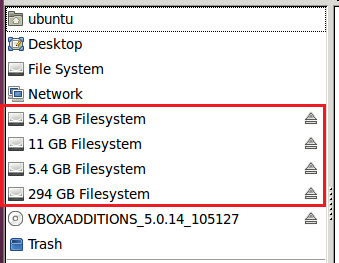
\includegraphics[width=0.9\linewidth]{Sonoscape_Analyse/Anzahl_Festplatten}}

In Abbildung \ref{fig:run_all_app} ist ein Auszug zu sehen, von dem Skript das über das RAM Dateisystem aufgerufen wird. Dieses Skript ruft selbst weitere Skripte auf die zum Beispiel Software installieren, bestimmte Ethernet Konfigurationen einstellen oder andere Systemeigenschaften verändern. Für die Manipulation des boot Vorgangs ist vor allem die rot umrandete Zeile wichtig, denn diese startet ein weiteres Skript, das letztendlich die Ultraschallsoftware startet. Nachdem die Software gestartet wurde ist es nicht mehr möglich weitere Befehle auf dem Betriebssystem auszuführen.\\

\section{Root Zugriff}

\begin{wrapfigure}{r}{0.5\textwidth}
\centering  	
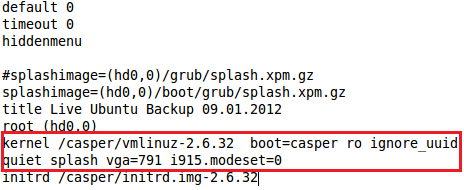
\includegraphics[width=0.5\textwidth]{Sonoscape_Analyse/grub_conf} 
		\caption{{\small Auszug aus der grub.conf Datei}}
		\label{fig:grub_conf}
\end{wrapfigure}
Um Änderungen auf dem SonoScape System vorzunehmen ist ein Terminal mit root Rechten erforderlich. Deswegen wurde zuerst versucht in ein Terminal zu booten statt des Betriebssystems. Damit sich vor dem booten ein Terminal öffnet müssen die boot Einstellungen des boot loaders grub modifiziert werden. Dazu müssen in der grub.conf Datei (siehe Abbildung \ref{fig:grub_conf}) einige Änderungen vorgenommen werden. Zuerst ist es notwendig den hiddenmenu Befehl zu löschen, damit der boot loader im boot Menü sichtbar wird.
Danach muss die rot markierte Zeile gelöscht werden, denn diese ist für das booten des RAM Dateisystems verantwortlich. Zum Schluss muss 
\shellcmd{grubterminal console} in die Datei geschrieben werden. Durch diesen Befehl kann direkt in das Terminal gebootet werden. Sind diese Änderungen abgeschlossen ist es möglich über das grub Bootmenü schließlich ein Terminal aufzurufen.\\
Dieses Terminal hat zwar root Rechte, jedoch befindet es sich nicht im echten Dateisystem sondern in dem Dateisystem des Arbeitsspeichers. Das hat zur Folge, dass nicht auf das persistente Dateisystem zugegriffen werden kann. Also ist es nicht möglich über dieses Terminal relevante Änderungen durchzuführen.
Der zweite Versuch hingegen basierte auf der Systemstruktur. Dafür wird genau auf das \textit{run all app} Skript eingegangen. In Abbildung \ref{fig:run_all_app} bedeutet der rot umrandete Kasten, dass die Ultraschallsoftware über ein weiteres Skript gestartet wird. Nach dem Auskommentieren rot umrandeten Zeile und dem neu Einfügen der Zeile \shellcmd{gnome -terminal} wird nicht nur der Start der Ultraschallsoftware verhindert, sondern auch ein Terminal geöffnet. Da das Skript \textit{run all app} mit root Rechten aufgerufen wird, hat auch das Terminal das in dem Skript aufgerufen wird automatisch ebenfalls root Rechte.

\section{Netzwerk Verbindung}

Aus den funktionalen Anforderungen (siehe Kapitel \ref{FunkAnf} ergibt sich die Notwendigkeit das SonoScape Gerät mit einem Smartphone zu verbinden. Im besten Fall kann die Verbindung direkt zwischen Smartphone und SonoScape Gerät aufgebaut werden. Dazu muss das Smartphone einen Hotspot aufmachen, zu dem sich das SonoScape Gerät über ein Ethernet Kabel oder über WLAN verbinden kann. Da ein Kabel zwischen Smartphone und SonoScape Gerät, die Benutzung des Ultraschallkopfes umständlicher macht, fällt die Kabelvariante raus.\\
Für eine kabellose Verbindung zwischen Ultraschallgerät und mobilen Endgerät muss eine Konfiguration für die Verwendung eines WLAN-Adapters vorgenommen werden..\\\\
\begin{large}
\textbf{WLAN Adapter}\\\\
\end{large}
Das Betriebssystem des SonoScapes ist ein Ubuntu 10.4 32 bit in einer modifizierten, abgespeckten Version. Dementsprechend sind keine Treiber für neuartige WLAN Adapter vorinstalliert. Deswegen muss ein Treiber für einen WLAN Adapter nachinstalliert werden. Das Problem dabei ist nur, dass die Treiber auf bestimmte Kernelfunktionalitäten zugreifen, die in der modifizierten Variante des Betriebssystems nicht enthalten sind. Der Kernel ist also inkompatibel mit aktueller Treiber Software. Um dieses Problem zu lösen muss ein relativ alter WLAN Adapter benutzt werden, da Ubuntu schon viele Treiber standardmäßig vorinstalliert hat. \\
Nachdem der WLAN Adapter erkannt ist, muss nur noch eine Verbindung zwischen Smartphone und SonoScape Gerät aufgebaut werden. Weil der Adapter nicht automatisch konfiguriert wird, muss er manuell über die Konsole konfiguriert werden. Trotzdem war es nicht möglich das vom Smartphone aufgespannte Netz zu erkennen. Denn der Ubuntu interne Netzwerk Manager revidierte die Konfigurationen sofort wieder oder ließ die Abspeicherung nicht zu. Nachdem Hinweis von Herrn Spiecher über das Abschalten des Netzwerk Managers funktionierte der relativ alte WLAN Adapter nach der Konfiguration problemlos. Schließlich kann das Smartphone direkt mit dem SonoScape verbunden werden.\\
Das Problem bei diesem Ansatz ist der alte WLAN Stick. Die Übertragungsrate ist so gering, dass nach verschiedenen Tests nur maximal zwei Bilder pro Sekunde übertragen werden konnten. Da in Kapitel \ref{FunkAnf} eine angemessene Anzahl von Bildern pro Sekunde gefordert ist, erfüllt der Ansatz nicht die aufgestellten Anforderungen.\\\\
\begin{large}
\textbf{Router}\\\\
\end{large}
Die letzte verbleibende Möglichkeit das Smartphone mit dem SonoScape zu verbinden, ist einen Router zu benutzen. Denn ein Router spannt ein eigenes Netzwerk auf, über das sich SonoScape und Smartphone separat mit dem Router verbinden können. Das SonoScape kann über ein Ethernet Kabel mit dem Router verbunden werden und das Smartphone über WLAN. So wird die Benutzbarkeit des Handspiegels nicht eingeschränkt und die Datenrate beträgt ca. 12-30 Bilder pro Sekunde, was den funktionalen Anforderungen gerecht wird. Der einzige Nachteil ist das zusätzliche Gerät und der damit verbundene Anschlussaufwand, der aber in Kauf genommen werden muss.\\
Die Vorkonfiguration des SonoScapes beinhaltet auch eine Netzwerkkonfiguration. Diese gibt dem SonoScape standardmäßig eine IP-Adresse von 172.22.16.180. Damit die IP Adresse nicht über ein Skript geändert werden muss, wird die Router IP Adresse standardmäßig auf 172.22.16.1 verändert, sodass sich beide Geräte im gleichen Netzwerk befinden. Nun ist es möglich den Router über ein Ethernet Kabel direkt mit dem SonoScape zu verbinden. 




